\addcontentsline{toc}{subsection}{Introduction}
\subsection*{An Introduction to Limits}

\begin{longtable}[ht]{|C{2.5cm}|C{6.6cm}|C{1.75cm}|C{1.75cm}|C{1.75cm}|} 
    \hline  Function & Graph & $\displaystyle\lim_{x\to c^-}f(x)$ & $\displaystyle\lim_{x\to c^+}f(x)$ & $\displaystyle\lim_{x\to c}f(x)$ \\\hline
    $\displaystyle\lim_{x\to 2}2x+1$ & 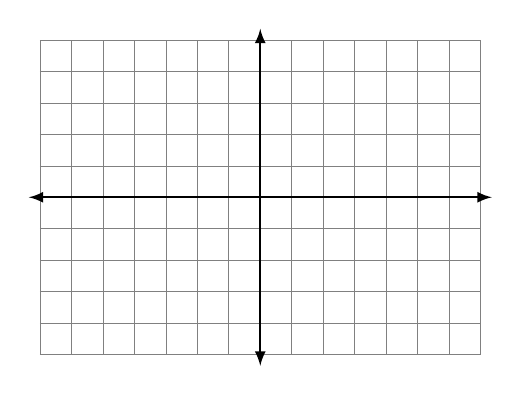
\begin{tikzpicture}[xscale=.4,yscale=.4]
          \draw[step=1,style=help lines,] (-7,-5) grid (7,5);
          \draw[latex-latex, thick] (-7.35,0)--(7.35,0);
          \draw[latex-latex, thick] (0,-5.35)--(0,5.35);
    \end{tikzpicture} & & & \\\hline
    $\displaystyle\lim_{x\to 0}x^2-2x+1$ & 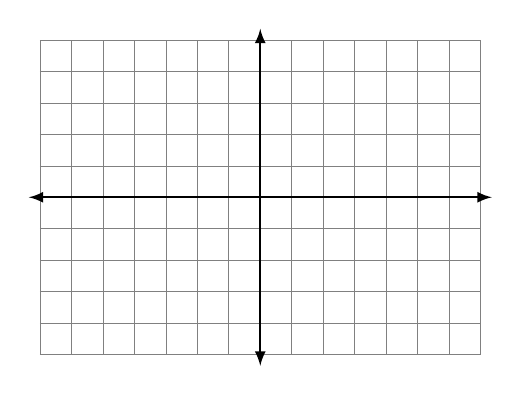
\begin{tikzpicture}[xscale=.4,yscale=.4]
          \draw[step=1,style=help lines,] (-7,-5) grid (7,5);
          \draw[latex-latex, thick] (-7.35,0)--(7.35,0);
          \draw[latex-latex, thick] (0,-5.35)--(0,5.35);
    \end{tikzpicture} & & & \\\hline
    $\displaystyle\lim_{x\to 2}\frac{x+3}{x+2}$ & 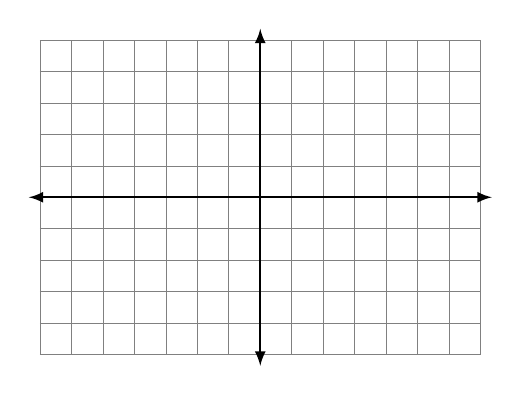
\begin{tikzpicture}[xscale=.4,yscale=.4]
          \draw[step=1,style=help lines,] (-7,-5) grid (7,5);
          \draw[latex-latex, thick] (-7.35,0)--(7.35,0);
          \draw[latex-latex, thick] (0,-5.35)--(0,5.35);
    \end{tikzpicture} & & & \\\hline
    $\displaystyle\lim_{x\to\frac{3\pi}{2}}\sin x$ & 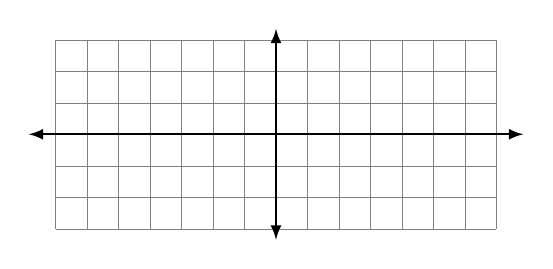
\begin{tikzpicture}[xscale=.4,yscale=.4]
          \draw[step=1,style=help lines,] (-7,-3) grid (7,3);
          \draw[latex-latex, thick] (-7.85,0)--(7.85,0);
          \draw[latex-latex, thick] (0,-3.35)--(0,3.35);
    \end{tikzpicture} & & & \\\hline
    $\displaystyle\lim_{x\to\pi}-3\cos\theta$ & 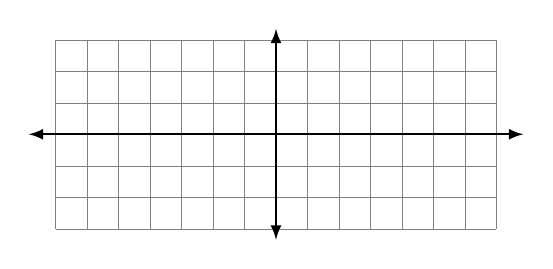
\begin{tikzpicture}[xscale=.4,yscale=.4]
          \draw[step=1,style=help lines,] (-7,-3) grid (7,3);
          \draw[latex-latex, thick] (-7.85,0)--(7.85,0);
          \draw[latex-latex, thick] (0,-3.35)--(0,3.35);
    \end{tikzpicture} & & & \\\hline
    $\displaystyle\lim_{x\to 5}\frac{x^2-25}{x-5}$ & 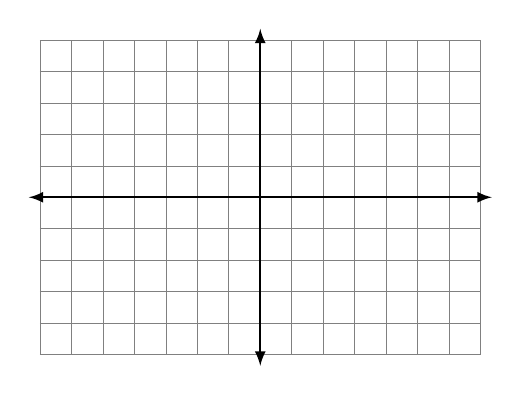
\begin{tikzpicture}[xscale=.4,yscale=.4]
          \draw[step=1,style=help lines,] (-7,-5) grid (7,5);
          \draw[latex-latex, thick] (-7.35,0)--(7.35,0);
          \draw[latex-latex, thick] (0,-5.35)--(0,5.35);
    \end{tikzpicture} & & & \\\hline
    $\displaystyle\lim_{x\to 5}|x+2|-1$ & 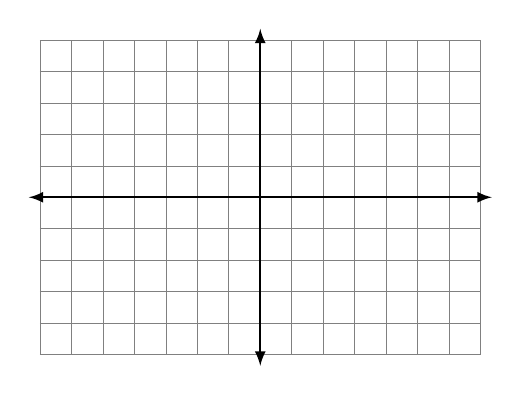
\begin{tikzpicture}[xscale=.4,yscale=.4]
          \draw[step=1,style=help lines,] (-7,-5) grid (7,5);
          \draw[latex-latex, thick] (-7.35,0)--(7.35,0);
          \draw[latex-latex, thick] (0,-5.35)--(0,5.35);
    \end{tikzpicture} & & & \\\hline
    $\displaystyle\lim_{x\to0}\frac{1}{x}$ & 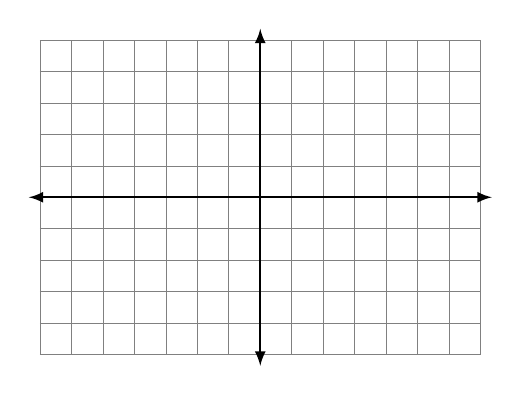
\begin{tikzpicture}[xscale=.4,yscale=.4]
          \draw[step=1,style=help lines,] (-7,-5) grid (7,5);
          \draw[latex-latex, thick] (-7.35,0)--(7.35,0);
          \draw[latex-latex, thick] (0,-5.35)--(0,5.35);
    \end{tikzpicture} & & & \\\hline
\end{longtable}
\vspace{\stretch{1}}
In short, we can interpret the limit as the expected $y$-value of a function. It doesn't really matter if the function even attains a the value the limit takes on. The behavior of the graph \textit{around} that point determines everything.
\vspace{\stretch{1}}

\newpage

\begin{tcolorbox}[title= DEFINITION OF THE EXISTENCE OF A LIMIT,colframe=black,sharp corners,colback=white,colbacktitle=white,coltitle=black,boxrule=1pt]

    A funciton has a limit as $x$ approaches $c$ if and only if the right hand limit and the left hand limit at a point $c$ are the same. That is
    
    \[\text{if }\lim_{x\to c^-}f(x)=\lim_{x\to c^+}f(x)=L,\,\text{then }\lim_{x\to c}=L.\]
\end{tcolorbox}
\vspace{.3cm}
\noindent There are three cases:
\begin{enumerate}
    \item A continuous function on the interval $(-\infty,
    ,\infty)$. \vspace{.75cm}
    \item A non-continuous function where $f(c)$ does not exist. \vspace{.75cm}
    \item A non-continuous function where $f(c)$ is defined at a different point.\vspace{.75cm}
\end{enumerate}

\noindent\textbf{Example:} Graph the function.\\
\begin{minipage}{0.30\linewidth}
    \[f(x)=
        \begin{cases}
        2-2x        &   [0,\,1)\\
        -(x-3)^2+2  &   [2,\,4)\\
        -1          &   4\\
        x-4         &   (4,\,5]
        \end{cases}
    \]
\end{minipage}
\hfill
\begin{minipage}{0.65\linewidth}
    \begin{center}
        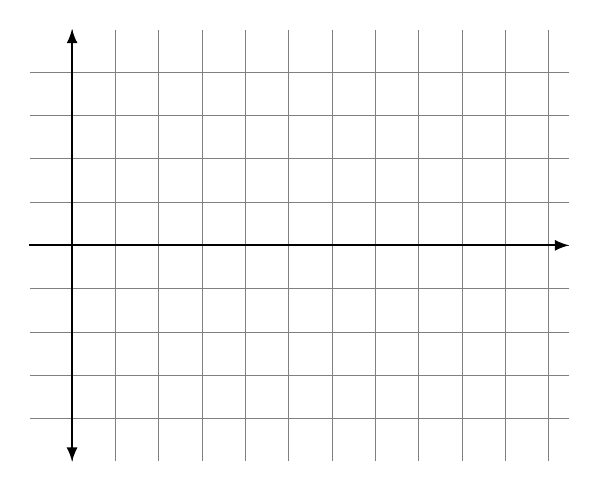
\begin{tikzpicture}[scale=1.1]
          \draw[step=.5,style=help lines] (-.49,-2.49) grid (5.74,2.49);
          \draw[-latex, thick] (-.5,0)--(5.74,0);
          \draw[latex-latex, thick] (0,-2.5)--(0,2.5);
    \end{tikzpicture}
    \end{center}
\end{minipage}

\begin{longtable}{|m{3.667cm}|m{3.667cm}|m{3.667cm}|m{3.7cm}|}
    \hline
    $\displaystyle f(0)=$   &   $\displaystyle\lim_{x\to0^+}f(x)=$  &   $\displaystyle\lim_{x\to0^-}f(x)=$  &   $\displaystyle\lim_{x\to0}f(x)=$ \\
                            &   &   &   \\\hline
    $\displaystyle f(1)=$   &   &   &   \\
                            &   &   &   \\\hline
    $\displaystyle f(2)=$   &   &   &   \\\
                            &   &   &   \\\hline
    $\displaystyle f(3)=$   &   &   &   \\\
                            &   &   &   \\\hline
    $\displaystyle f(4)=$   &   &   &   \\\
                            &   &   &   \\\hline
    $\displaystyle f(5)=$   &   &   &   \\
                            &   &   &   \\\hline
\end{longtable}

\newpage

A limit is the value of the function we \textbf{approach} as we near a particular $x$ from either the left or the right. A limit is \textbf{not} necessarily the value of the function at that point.
\vspace{\stretch{.15}}

\noindent\textbf{Strategies for Finding Limits:}
\begin{enumerate}
    \item Substitute in
    \item Simplify the equation algebraically, then substitute in
    \item Make the graph and determine the limit visually
    \item Construct a table of values to conjecture a limit
\end{enumerate}
\vspace{\stretch{.15}}
\noindent\textbf{Examples:}
\begin{questions}
    \question $\displaystyle\lim_{x\to3}\frac{x^2+1}{2x}$ \vspace{\stretch{1}}
    \question $\displaystyle\lim_{x\to2}\floor*{x}$ \vspace{\stretch{1}}
    \question $\displaystyle\lim_{x\to-4.1}\floor*{x}$ \vspace{\stretch{1}}
    \question $\displaystyle\lim_{x\to3}\frac{x^2-9}{x+3}$ \vspace{\stretch{1}}
    \question $\displaystyle\lim_{t\to2}\frac{t^2-3t+2}{t^2-4}$ \vspace{\stretch{1}}

\newpage

    \question $\displaystyle\lim_{x\to0}\frac{\frac{1}{2+x}-\frac{1}{2}}{x}$ \vspace{\stretch{1}}
    \question $\displaystyle\lim_{x\to0}\frac{(2+x)^3-8}{x}$ \vspace{\stretch{1}}
\end{questions}

